\chapter{Question 1}
\label{question-1}
\section{Question}

\begin{itemize}
\item Choose 100 URIs from A1.
\item Generate WARC files of those URIs using:
\begin{itemize}
\item wget
\item WARCreate
\item Heritrix (stand-alone or via WAIL)
\item webrecorder.io
\end{itemize}
\item Describe the resulting WARC files: quantitatively compare  contrast the results of the WARC files of the same URI as generated by different tools.
\begin{itemize}
\item choose interesting examples.
\end{itemize}
\item Demonstrate playback of 2-3 WARCs in the (Wayback Machine (via WAIL or stand-alone) or pywb) and (webrecorder.io)
\begin{itemize}
\item \hyperref[savePage]{https://github.com/iipc/openwayback}
\item \hyperref[savePage]{https://github.com/ikreymer/pywb}
\end{itemize}
\end{itemize}

\section{Solution}
\begin{itemize}
\item Fetching the 100 URIs was an arduous task, as a lot of the URIs had explicit content or were not accessible anymore. I had to open most of the links manually and as I progressed through the links I noticed a pattern and started avoiding those links to avoid additional time fetching the URIs.
\item I saved the URIs into a uri.txt file.
\item Soon after I installed the plug-in for WARCreate from Chrome Web Store and started manually visiting these URIs and clicking on the Warccreate button in the address bar for chrome web browser for downloading the WARC files.
\item After WARCreate, I moved onto the next tool webrecorder.io. I manually opened each of the URIs on the website and started downloading the WARC files. While fetching them manually I realized this activity could be automated but I decided that performing this task manually would re-assure me that the WARC files have been created properly.
\item The third tool WAIL consumed most of my time as the set-up wasn't as simple as it had multiple dependencies, required configuration changes and lacked proper documentation. As the thought of setting up stand-alone heritrix creeped into my mind, WAIL set-up issues were addressed by an email from Alexander Nwala and after following his instructions I was able to get the WAIL tool working.
\item I used the WAIL tool to create the archive but it took too long for most of the links so I put a time limit of approximately 10 minutes for each of the URIs and then manually stopped execution and moved to the next URI.
\item ``wget" was the simplest of all the tools for WARC creation. I used a simple unix command with the template ``wget URI --warc-file=FILENAME --no-warc-compression" for each of the 100 URIs.
\end{itemize}

\section{Comparison}
\begin{itemize}
\item From the 10000 URIs retrieved from the first assignment we took a sample of 100 URIs. To make a meaningful comparison of the sample I calculated the mean of the size of WARC files from each of the tools.
\item Below is the graph to represent the average size of the WARC files for each of the tools. \\*
	\begin{minipage}{\linewidth}
		\centering
		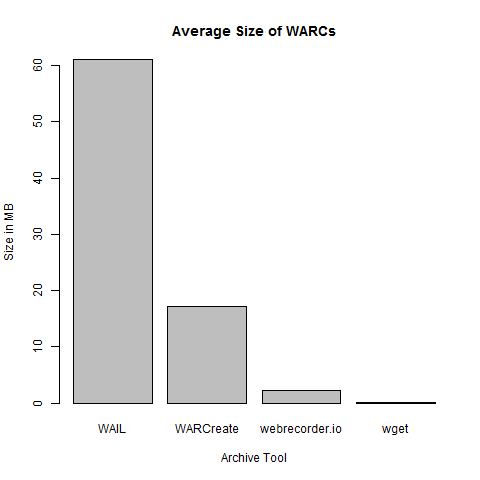
\includegraphics[scale=0.55]{figures/avgWarcSizeForTool.png}
		\captionof{figure}{Average Size of WARC file for sample size=100}
		\label{avgWarcSizeForTool}
	\end{minipage}

\item While downloading the WARC files for each of the above tools I noticed a trend that WAIL was able to crawl the deepest and it had to be manually stopped. The size of the files generated by WAIL were significantly larger than the ones created by the other tools.
\item With this information and the above graph I concluded that WAIL creates the largest of the files. Upon further analysis I found that WAIL crawls dereferences each of the URIs in the webpage. WAIL does not stop until it crawls to the end of the URI.
\item As it is a configurable tool, we can modify the specify the time spent to crawl each URI, maximum size of the WARC file and/or maximum documents downloaded in the crawler-beans.cxml created for each of the jobs.
\item Below are the WARC size plots for three randomly chosen URIs as specified below, which I've used for the rest of the assignment for playback demonstration.
	\begin{itemize}
	\item URI\#1: \hyperref[savePage]{http://edition.cnn.com/videos/us/2015/02/04/lead-dnt-johns-plane-crash-taiwan.cnn}
	\item URI\#2: \hyperref[savePage]{http://www.dccomics.com/blog/2015/02/04/breaking-news-milo-ventimiglia-is-coming-to-gotham}
	\item URI\#3: \hyperref[savePage]{http://www.theguardian.com/football/2015/feb/04/jonny-evans-manchester-united-louis-van-gaal}
	\end{itemize}
	\begin{minipage}{\linewidth}
		\centering
		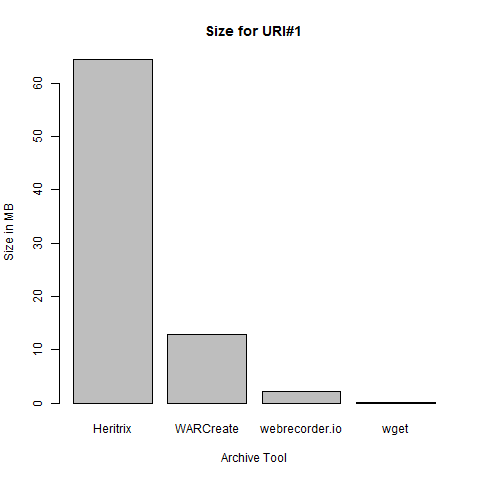
\includegraphics[scale=0.55]{figures/uri1.png}
		\captionof{figure}{Archive Tools vs. Size for URI\#1}
		\label{sizeURI1}
	\end{minipage}
	\begin{minipage}{\linewidth}
		\centering
		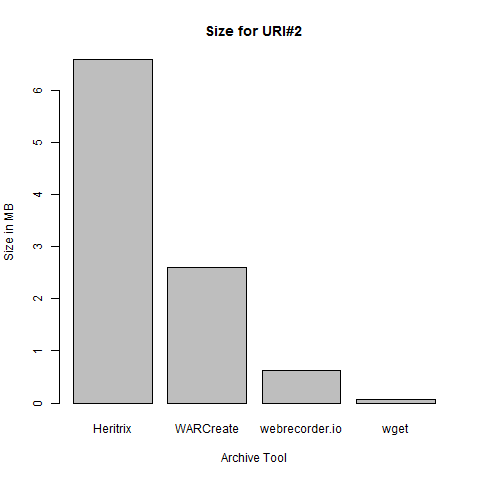
\includegraphics[scale=0.55]{figures/uri2.png}
		\captionof{figure}{Archive Tools vs. Size for URI\#2}
		\label{sizeURI2}
	\end{minipage}
	\newpage
	\begin{minipage}{\linewidth}
		\centering
		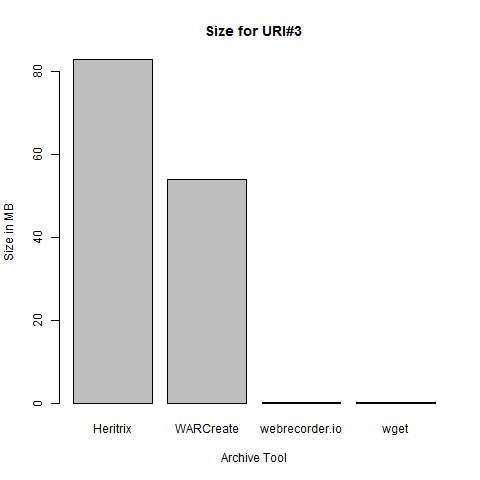
\includegraphics[scale=0.55]{figures/uri3.png}
		\captionof{figure}{Archive Tools vs. Size for URI\#3}
		\label{sizeURI3}
	\end{minipage}
\end{itemize}

\section{Playback}
\subsection{Webrecorder.io}
\begin{minipage}{\linewidth}
	
\includegraphics[scale=0.55]{figures/playback/webrecorder_7_wail.PNG}
	\captionof{figure}{Web Recorder - WAIL generated WARC for URI\#1}
	\label{webrecorder_7_wail}
\end{minipage}
\newpage
\begin{minipage}{\linewidth}
	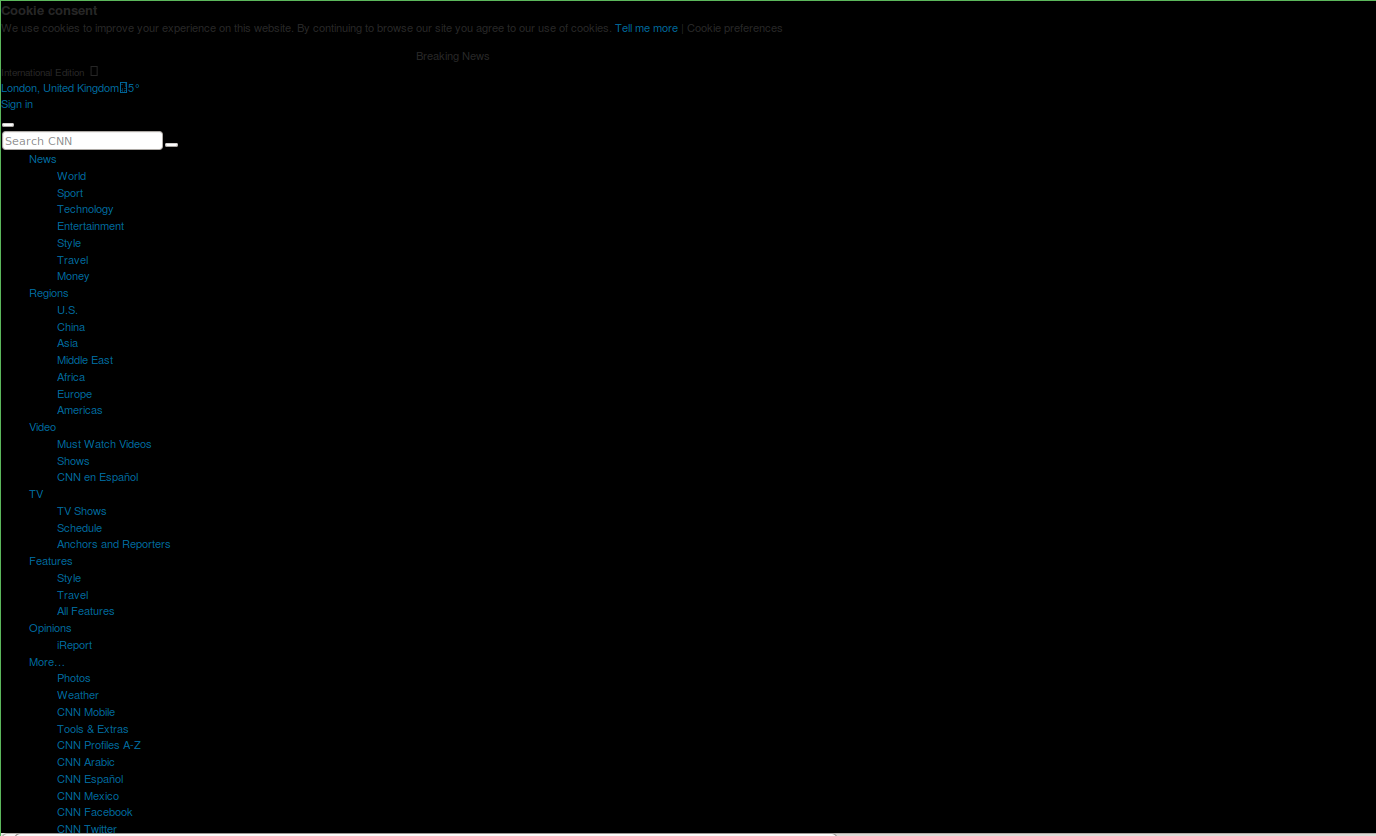
\includegraphics[scale=0.55]{figures/playback/webrecorder_7_warcreate.PNG}
	\captionof{figure}{Web Recorder - WARCreate generated WARC for URI\#1}
	\label{webrecorder_7_warcreate}
\end{minipage}
\newpage
\begin{minipage}{\linewidth}
	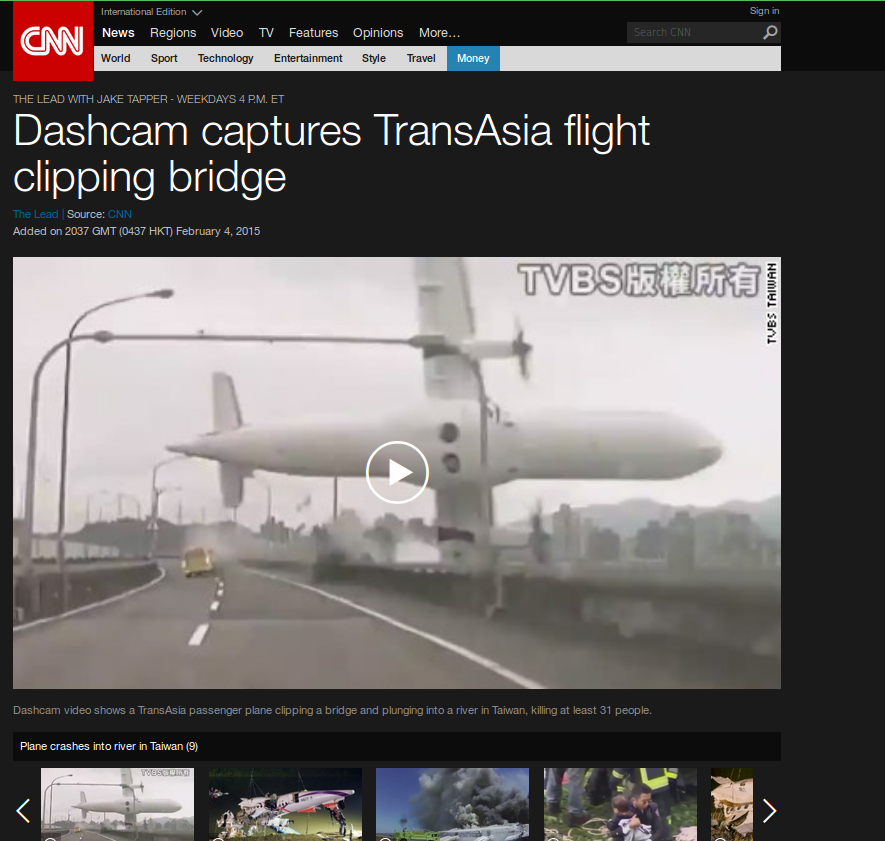
\includegraphics[scale=0.55]{figures/playback/webrecorder_7_webrecorder.PNG}
	\captionof{figure}{Web Recorder - webrecorder.io generated WARC for URI\#1}
	\label{webrecorder_7_webrecorder}
\end{minipage}
\newpage
\begin{minipage}{\linewidth}
	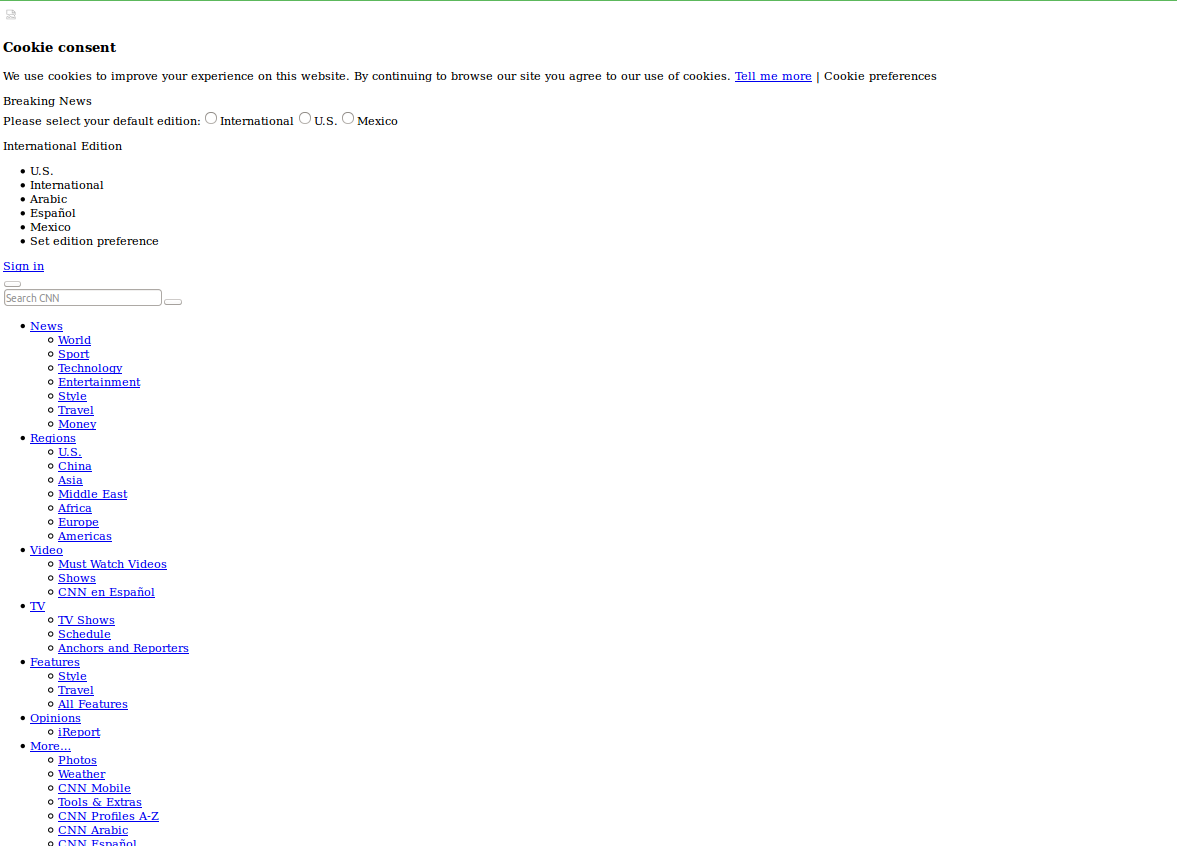
\includegraphics[scale=0.55]{figures/playback/webrecorder_7_wget.PNG}
	\captionof{figure}{Web Recorder - wget generated WARC for URI\#1}
	\label{webrecorder_7_wget}
\end{minipage}
\newpage
\begin{minipage}{\linewidth}
	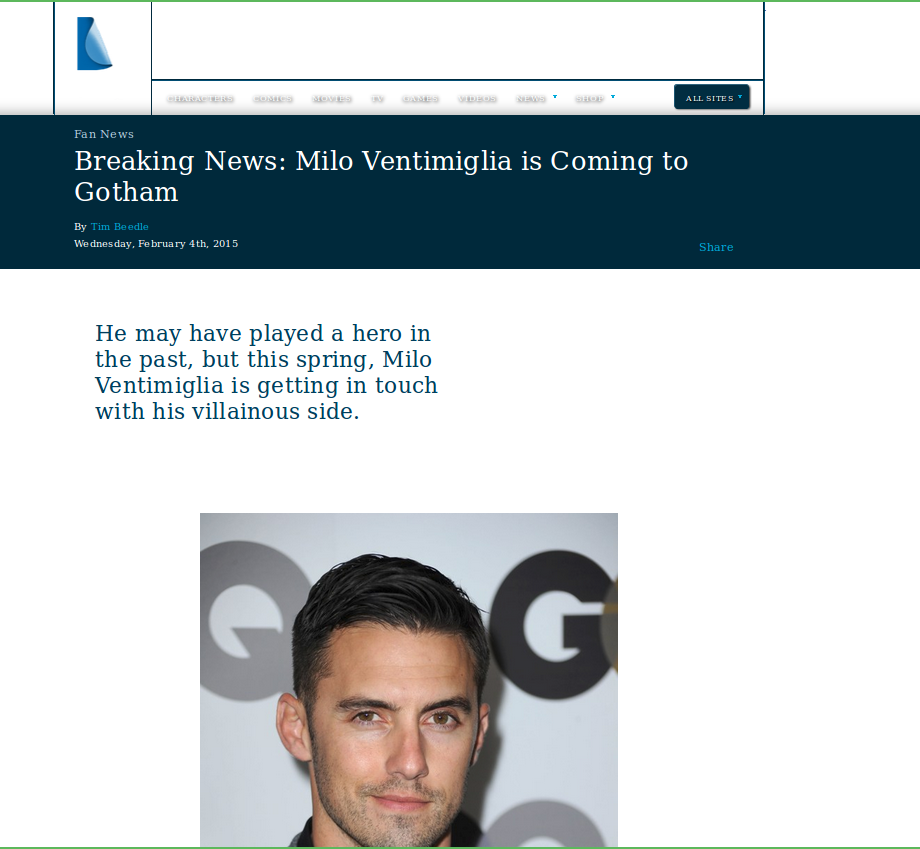
\includegraphics[scale=0.55]{figures/playback/webrecorder_24_wail.PNG}
	\captionof{figure}{Web Recorder - WAIL generated WARC for URI\#1}
	\label{webrecorder_24_wail}
\end{minipage}
\newpage
\begin{minipage}{\linewidth}
	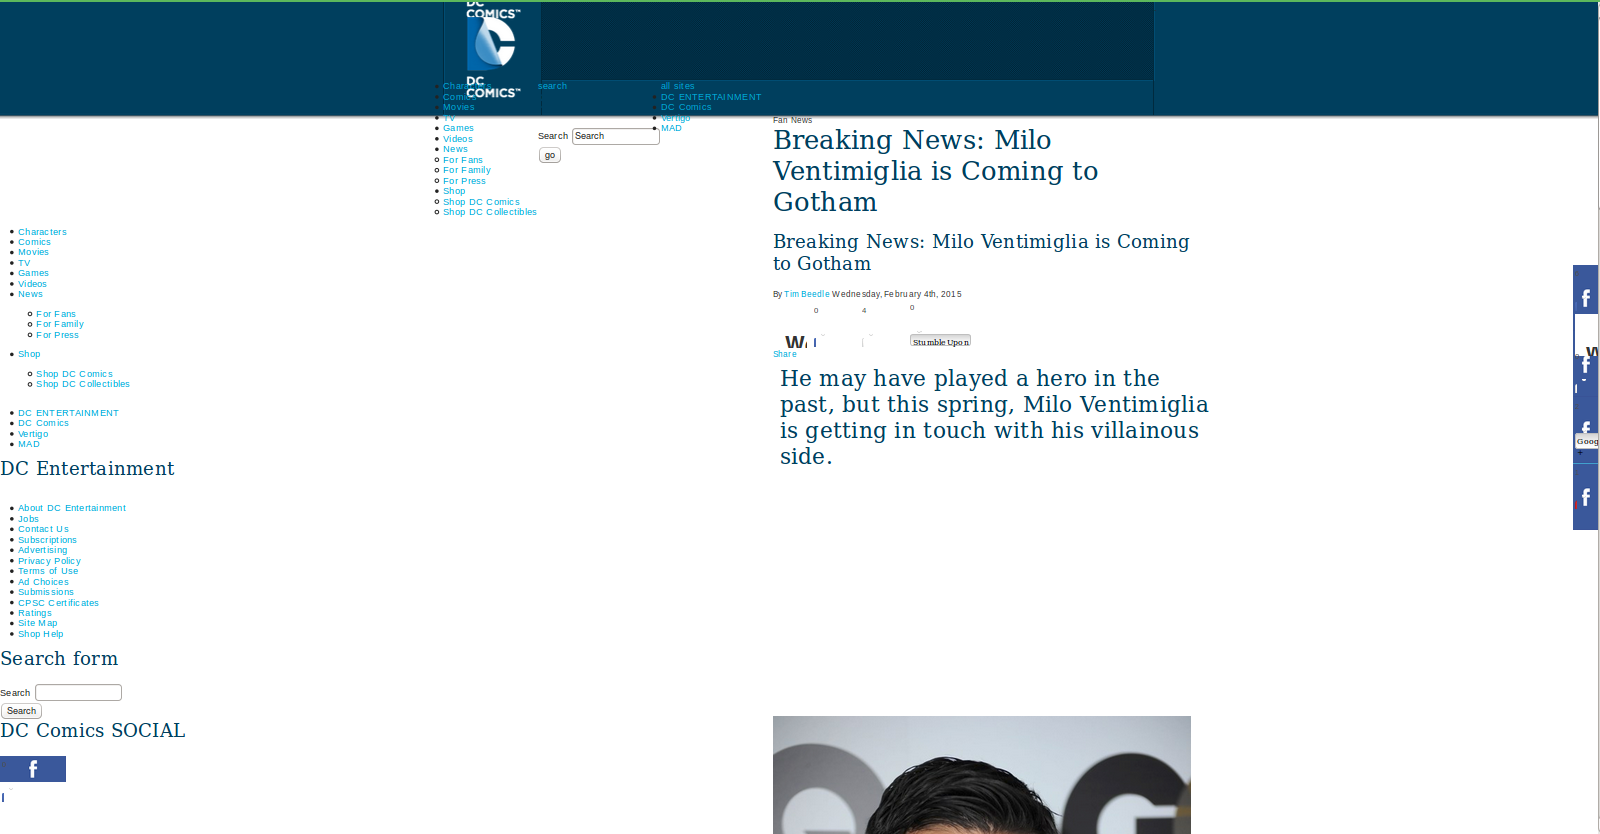
\includegraphics[scale=0.55]{figures/playback/webrecorder_24_warcreate.PNG}
	\captionof{figure}{Web Recorder - WARCreate generated WARC for URI\#1}
	\label{webrecorder_24_warcreate}
\end{minipage}
\newpage
\begin{minipage}{\linewidth}
	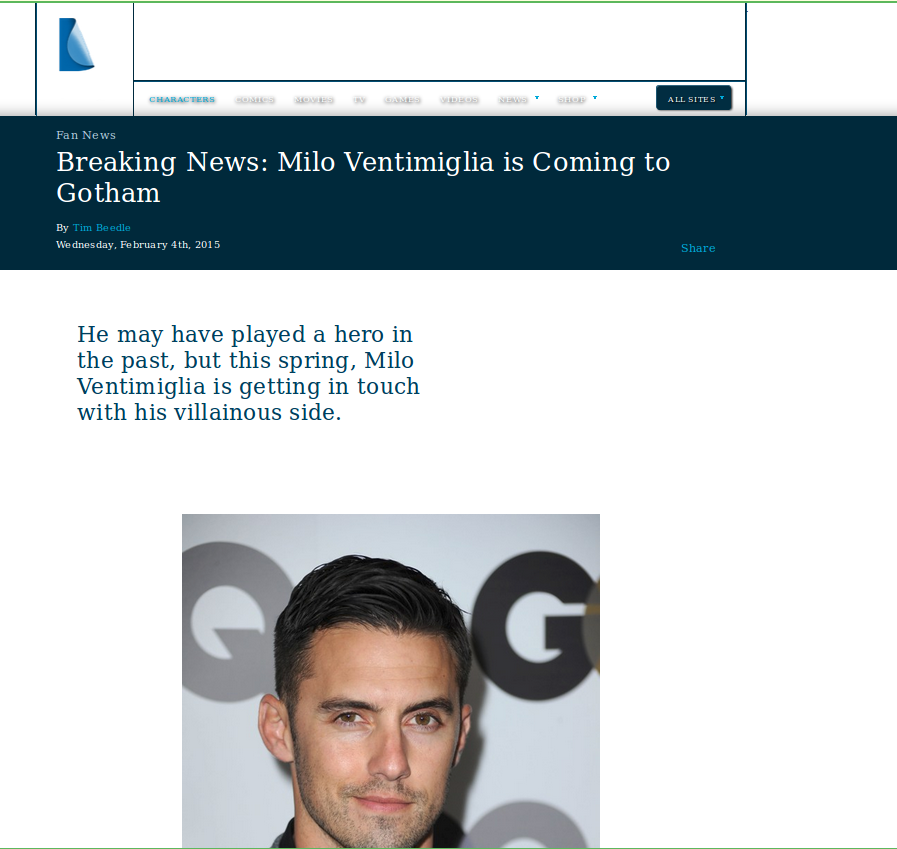
\includegraphics[scale=0.55]{figures/playback/webrecorder_24_webrecorder.PNG}
	\captionof{figure}{Web Recorder - webrecorder.io generated WARC for URI\#1}
	\label{webrecorder_24_webrecorder}
\end{minipage}
\newpage
\begin{minipage}{\linewidth}
	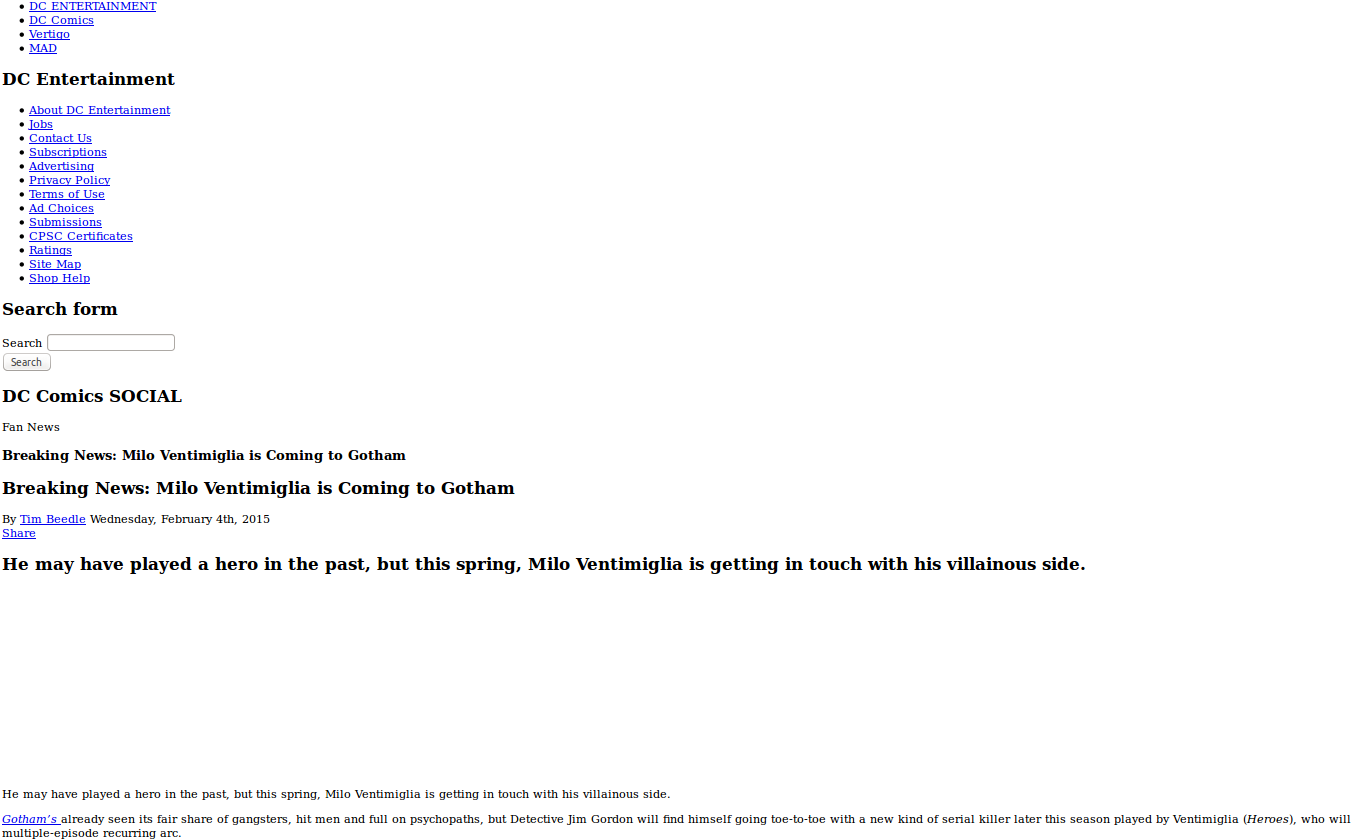
\includegraphics[scale=0.55]{figures/playback/webrecorder_24_wget.PNG}
	\captionof{figure}{Web Recorder - wget generated WARC for URI\#1}
	\label{webrecorder_24_wget}
\end{minipage}
\newpage
\begin{minipage}{\linewidth}
	
\includegraphics[scale=0.55]{figures/playback/webrecorder_89_wail.PNG}
	\captionof{figure}{Web Recorder - WAIL generated WARC for URI\#1}
	\label{webrecorder_89_wail}
\end{minipage}
\newpage
\begin{minipage}{\linewidth}
	
\includegraphics[scale=0.55]{figures/playback/webrecorder_89_warcreate.PNG}
	\captionof{figure}{Web Recorder - WARCreate generated WARC for URI\#1}
	\label{webrecorder_89_warcreate}
\end{minipage}
\newpage
\begin{minipage}{\linewidth}
	
\includegraphics[scale=0.55]{figures/playback/webrecorder_89_webrecorder.PNG}
	\captionof{figure}{Web Recorder - webrecorder.io generated WARC for URI\#1}
	\label{webrecorder_89_webrecorder}
\end{minipage}
\newpage
\begin{minipage}{\linewidth}
	
\includegraphics[scale=0.55]{figures/playback/webrecorder_89_wget.PNG}
	\captionof{figure}{Web Recorder - wget generated WARC for URI\#1}
	\label{webrecorder_89_wget}
\end{minipage}
\newpage

\subsection{pywb}
\begin{itemize}
\item For setting pywb I followed the instructions at \hyperref[savePage]{https://github.com/ikreymer/pywb}.
\item I created the cdx files for the WARC files and then launched pywb using the command wayback after going to the root folder of pywb in the terminal.
\item I used the web browser and went to "localhost:8080" for accessing the web interface for pywb. Below is the search interface for pywb. 
\end{itemize}
\begin{minipage}{\linewidth}
	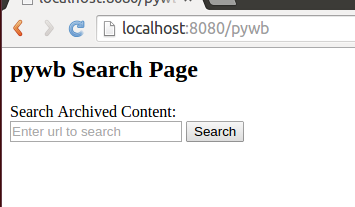
\includegraphics[scale=0.55]{figures/playback/search.PNG}
	\centering
	\captionof{figure}{Web Search Interface pywb}
	\label{search}
\end{minipage}
\begin{itemize}
\item After creating the cdx files for the associated URIs, enter the URI in the search field.
\item I was facing an issue with the WAIL results not being displayed for pywb inspite of the cdx files being generated properly and no errors in the command prompt. I tried using different WAIL generated WARC files but I was still not able to view it in the list of search results and hence wasn't able to display the results.
\end{itemize}
\begin{minipage}{\linewidth}
	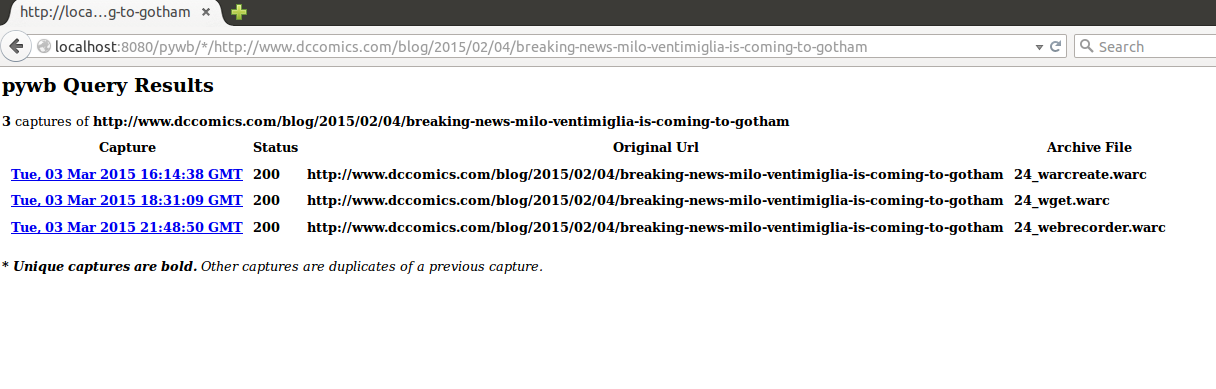
\includegraphics[scale=0.55]{figures/playback/pywb_search_page.PNG}
	\centering	
	\captionof{figure}{Search results page on pywb}
	\label{pywb_search_page}
\end{minipage}
\newpage
\begin{minipage}{\linewidth}
	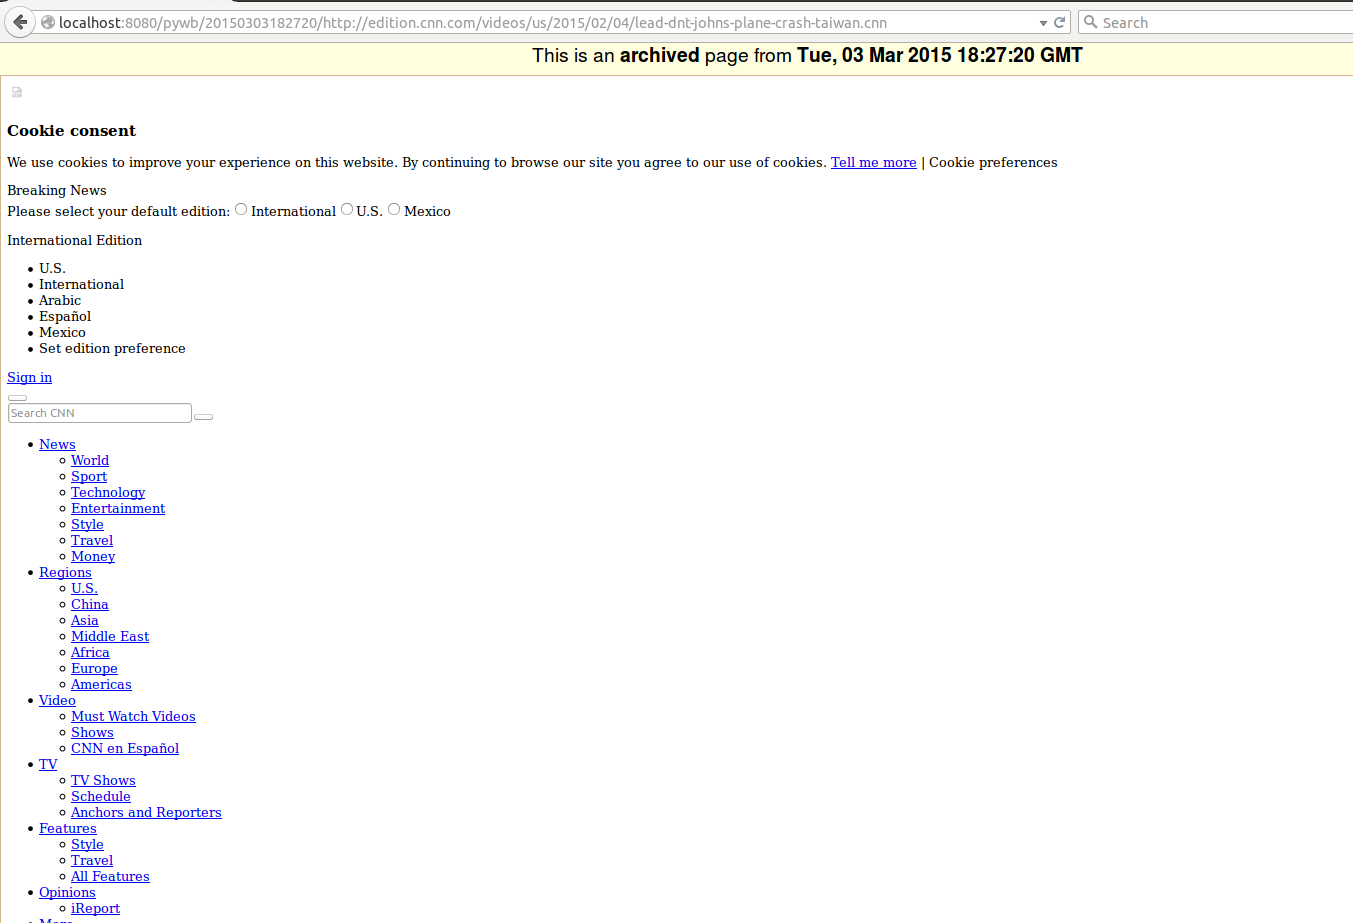
\includegraphics[scale=0.55]{figures/playback/pywb_7_wget.PNG}
	\captionof{figure}{pywb - wget generated WARC for URI\#1}
	\label{sizeURI3}
\end{minipage}
\newpage
\begin{minipage}{\linewidth}
	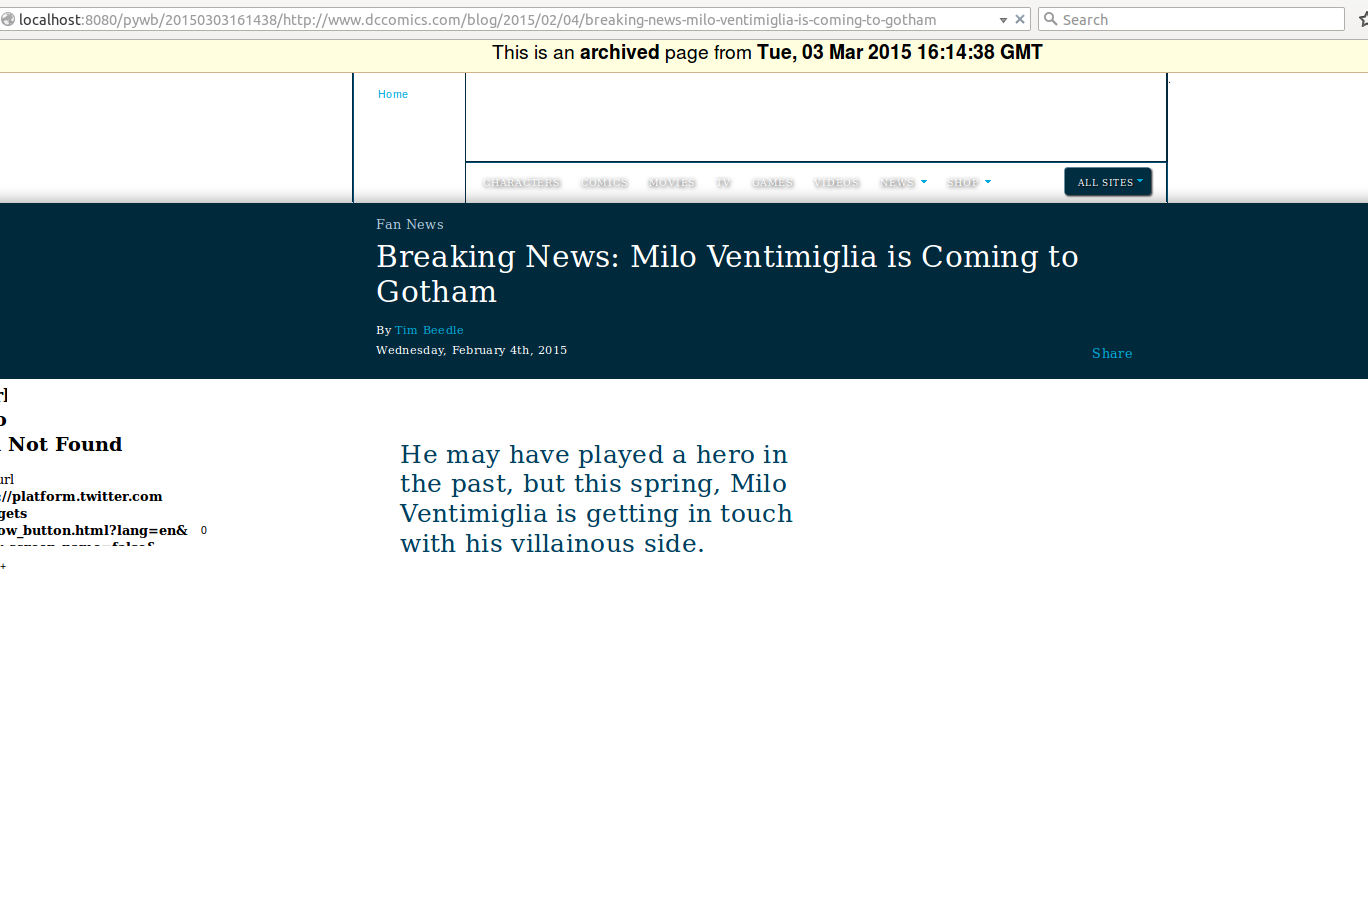
\includegraphics[scale=0.55]{figures/playback/pywb_24_warcreate.PNG}
	\captionof{figure}{pywb - WARCreate generated WARC URI\#2}
	\label{sizeURI3}
\end{minipage}
\newpage
\begin{minipage}{\linewidth}
	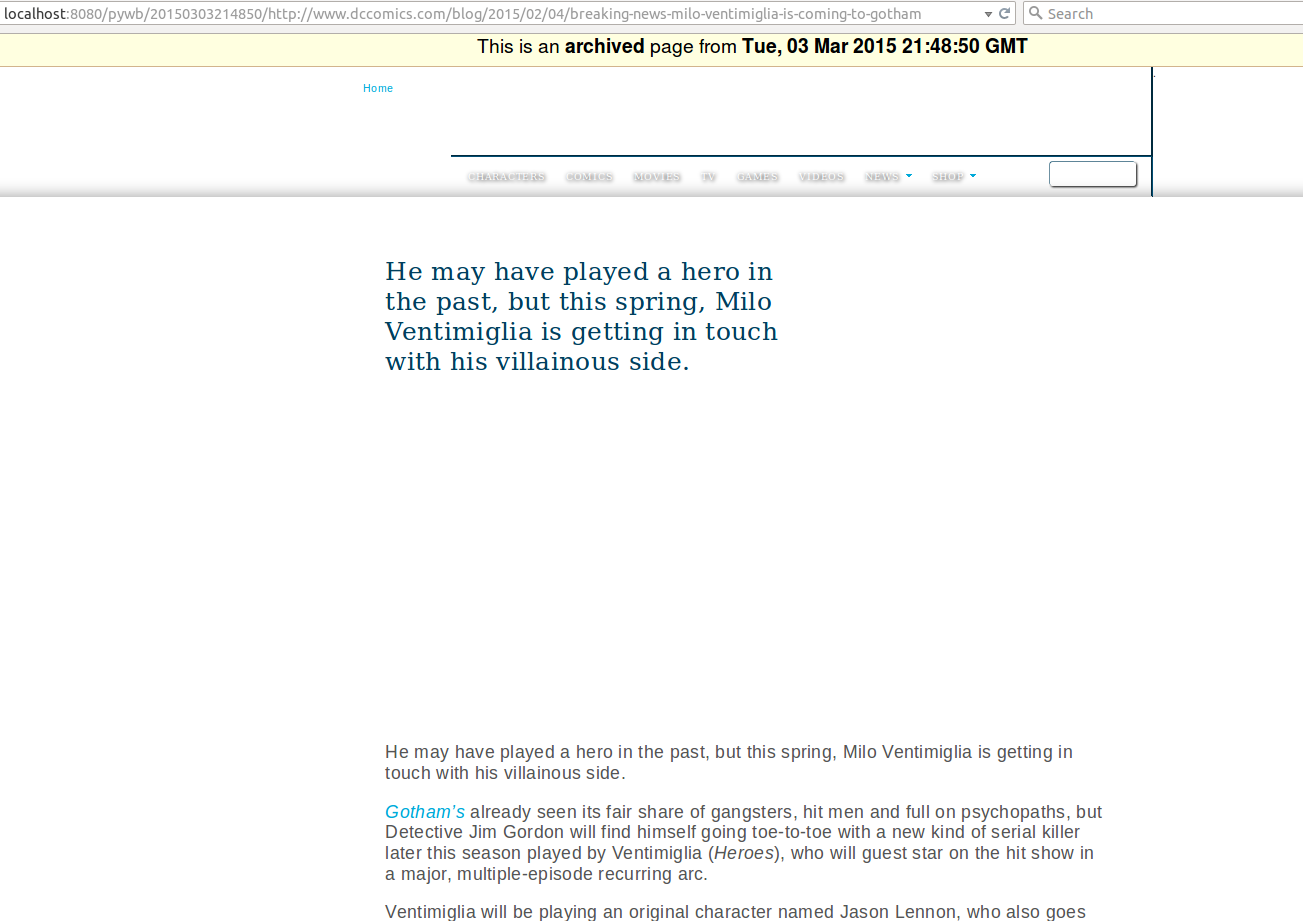
\includegraphics[scale=0.55]{figures/playback/pywb_24_webrecorder.PNG}
	\captionof{figure}{pywb - webrecorder.io generated WARC URI\#2}
	\label{sizeURI3}
\end{minipage}
\newpage
\begin{minipage}{\linewidth}
	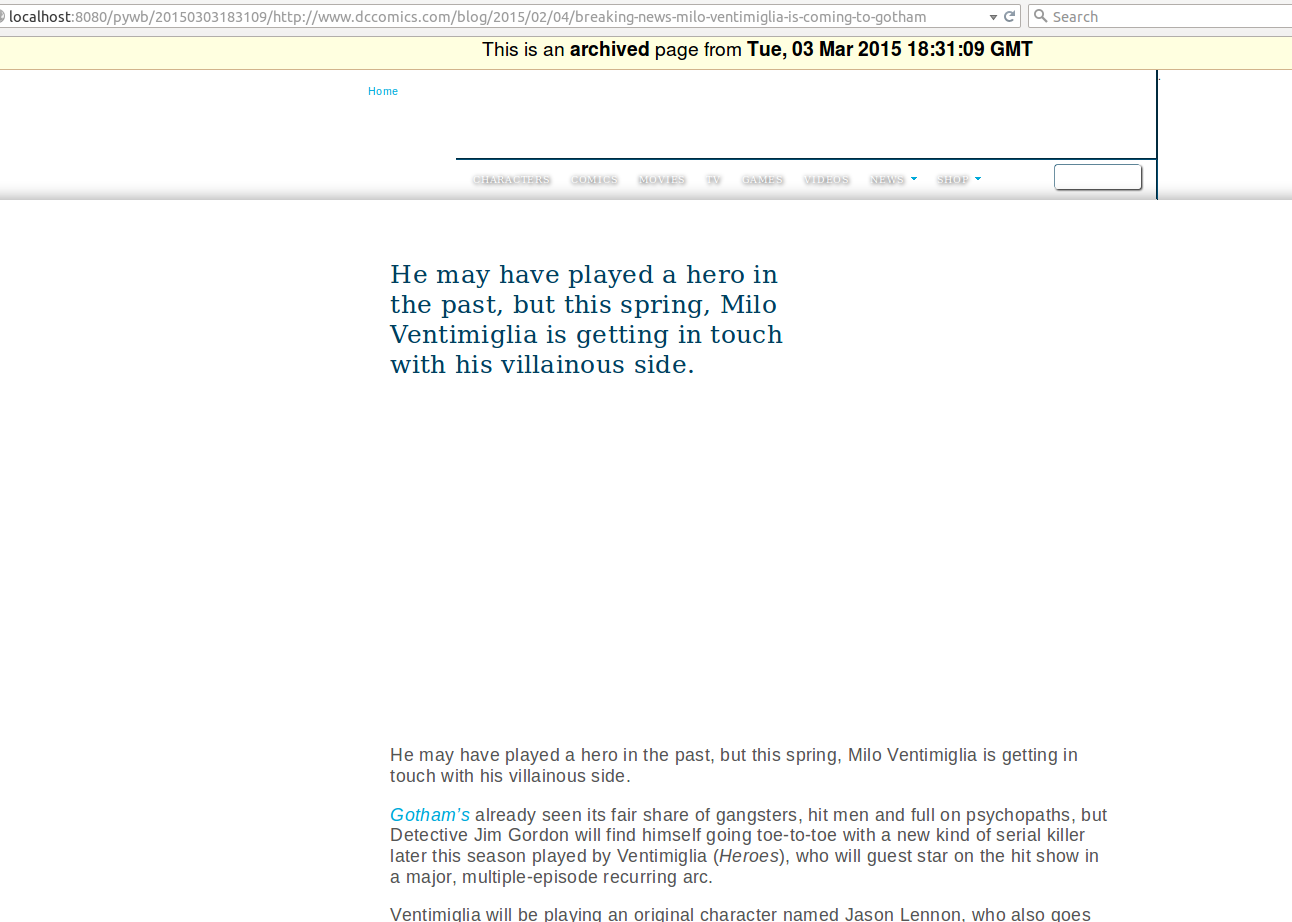
\includegraphics[scale=0.55]{figures/playback/pywb_24_wget.PNG}
	\captionof{figure}{pywb - wget generated WARC URI\#2}
	\label{sizeURI3}
\end{minipage}
\newpage
\begin{minipage}{\linewidth}
	
\includegraphics[scale=0.55]{figures/playback/pywb_89_webrecorder.PNG}
	\captionof{figure}{pywb - webrecorder.io generated WARC URI\#3}
	\label{sizeURI3}
\end{minipage}
\newpage
\begin{minipage}{\linewidth}
	
\includegraphics[scale=0.55]{figures/playback/pywb_89_wget.PNG}
	\captionof{figure}{pywb - wget generated WARC URI\#3}
	\label{sizeURI3}
\end{minipage}

\newpage
\section{Code Listing}
\lstinputlisting[language=R,breaklines = true,frame=single,caption={R program for generating the bar plot for WARC Tools vs. Average Size of WARC files for 100 samples}, label=lst:q1R1,captionpos=b,numbers=left,showspaces=false,showstringspaces=false,basicstyle=\footnotesize]{rFiles/barplot.R}